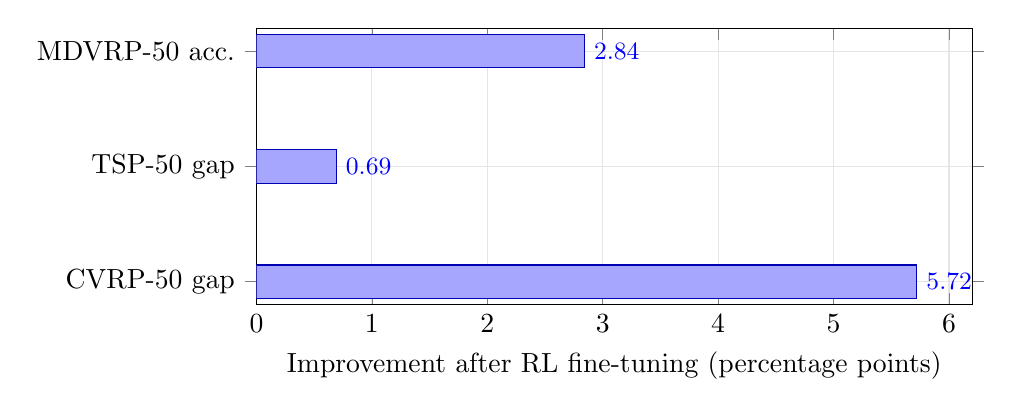
\begin{tikzpicture}
\begin{axis}[
  width=0.88\textwidth,
  height=0.42\textwidth,
  xbar,
  xmin=0,
  xmax=6.2,
  xlabel={Improvement after RL fine-tuning (percentage points)},
  symbolic y coords={MDVRP-50 acc.,TSP-50 gap,CVRP-50 gap},
  ytick=data,
  y dir=reverse,
  nodes near coords,
  nodes near coords align={horizontal},
  every node near coord/.append style={font=\small},
  grid=both,
  grid style={draw=gray!20},
  bar width=12pt,
]
\addplot+[fill=blue!35, draw=blue!70!black] coordinates {
  (0.69,TSP-50 gap)
  (5.72,CVRP-50 gap)
  (2.84,MDVRP-50 acc.)
};
\end{axis}
\end{tikzpicture}
